% 124-16(124쪽) — $y=\tan(ax-b)$ 의 그래프와 점근선(점선 $x=-\frac{\pi}{2}$, $x=\frac{\pi}{2}$, $x=\pi$ · $x=0$ 은 $y$축이 대신한다).
% 스캔 화질이 낮아 TikZ 로 다시 그림. 원문에 있는 라벨만 둔다 — 축 위쪽 $-\frac{\pi}{4}$, $\frac{\pi}{4}$, $\frac{3}{4}\pi$(곡선의 $x$절편)와
% 축 아래쪽 $-\frac{\pi}{2}$, $\frac{\pi}{2}$, $\pi$(점근선). $y$축 눈금과 $a$, $b$ 의 값은 원문에 없으므로 넣지 않는다.
% 눈금 라벨은 곡선 가지 사이의 빈 자리에 들어가야 해서 \footnotesize(원문도 본문보다 작은 활자다).
\begin{tikzpicture}[line width=0.6pt, x=0.75cm, y=0.40cm]
  \draw[dotted, line width=0.5pt] (-1.5708,-3.3) -- (-1.5708,3.3);
  \draw[dotted, line width=0.5pt] (1.5708,-3.3) -- (1.5708,3.3);
  \draw[dotted, line width=0.5pt] (3.1416,-3.3) -- (3.1416,3.3);
  \draw[->, >=stealth, line width=0.7pt] (-2.45,0) -- (4.35,0) node[below=1pt] {$x$};
  \draw[->, >=stealth, line width=0.7pt] (0,-3.5) -- (0,3.9) node[left=1pt] {$y$};
  \draw[domain=-2.23:-1.7318, samples=50, smooth] plot (\x, {tan(114.5916*\x-90)});
  \draw[domain=-1.4100:-0.1610, samples=70, smooth] plot (\x, {tan(114.5916*\x-90)});
  \draw[domain=0.1610:1.4100, samples=70, smooth] plot (\x, {tan(114.5916*\x-90)});
  \draw[domain=1.7318:2.9806, samples=70, smooth] plot (\x, {tan(114.5916*\x-90)});
  \draw[domain=3.3026:3.80, samples=50, smooth] plot (\x, {tan(114.5916*\x-90)});
  \node[anchor=south east, font=\footnotesize] at (-0.72,0.10) {$-\dfrac{\pi}{4}$};
  \node[anchor=south east, font=\footnotesize] at (0.84,0.10) {$\dfrac{\pi}{4}$};
  \node[anchor=south east, font=\footnotesize] at (2.42,0.10) {$\dfrac{3}{4}\pi$};
  \node[anchor=north east, font=\footnotesize] at (-1.55,-0.10) {$-\dfrac{\pi}{2}$};
  \node[anchor=north east, font=\footnotesize] at (1.55,-0.10) {$\dfrac{\pi}{2}$};
  \node[anchor=north east, font=\footnotesize] at (3.12,-0.10) {$\pi$};
  \node[anchor=north east, font=\footnotesize] at (-0.04,-0.10) {$\pt{O}$};
  \node[anchor=south west, font=\small] at (0.28,3.25) {$y=\tan (ax-b)$};
\end{tikzpicture}
